\documentclass[12pt]{article}
\usepackage[a4paper, margin=.30in]{geometry}
\usepackage{graphicx ,
            wrapfig,
            xcolor, 
            enumerate,
            amsmath,
            comment
            }

\newcommand\headerMe[2]{\noindent{}#1\hfill#2}
\renewcommand{\thesection}{\Roman{section}}

\title{Leçon N 2 : Travail et puissance d’une force }
\author{Zakaria HAOUZAN}
\date{\today}

\begin{document}
% headers --------------
\headerMe{Matière : Physique-Chimie}{Professeur : Zakaria HAOUZAN}\\
\headerMe{Unité : la chimie autour de nous}{Établissement : Lycée SKHOR qualifiant}\\
\headerMe{Niveau : 1BAC S-SM}{Heure : 4H}\\

% ------Content ________
\begin{center}

    \Large{Leçon N4: \color{red}SUIVI D’UNE TRANSFORMATION \\CHIMIQUE}
\end{center}
\begin{comment}
\section{Introduction}

\begin{wrapfigure}{r}{0.25\textwidth}
    \centering
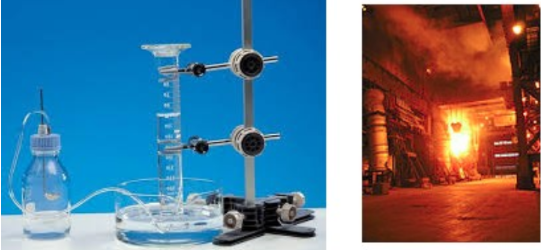
\includegraphics[width=0.25\textwidth]{./img/img00.png}
\end{wrapfigure} 
La première photo montre un dispositif expérimental permet de mesurer le volume du gaz récupérer au cours d’une transformation
chimique . Dans la deuxième photo nous observons une réaction du fer fondu avec le dioxygène qui produit des gerbes de lumière.
\\
\textbf{-Comment Le chimiste réalise-t-il des transformations chimiques
pour obtenir de nouveau corps?}\\\textbf{-Comment Le chimiste peut-il suivre des transformations
chimiques ?}
\end{comment}
%__________sub_Section 1 _______________
\section{ Transformation chimique–réaction chimique :}
    \subsection{Transformation chimique}
        \textbf{Au cours d’une transformation chimique des substances disparaissent et d’autres nouvelles substances apparaissent.}\\
Une transformation chimique peut être modélisée par une réaction chimique :
\begin{itemize}
    \item Les substances qui disparaissent sont appelées \underline {les réactifs.}
    \item Les substances qui apparaissent sont appelées \underline{les produits.}
\end{itemize}
\textbf{On appelle système chimique l’ensemble des éléments chimiques existant dans le milieu réactionnel.}


%______________sub___Section 2_______________________________
\subsection{ Etat initial et état final :}
    \textbf{La transformation chimique représente le passage d’un système chimique d’un état initial à un état final}
\begin{itemize}
    \item On appelle état initial, l’état du système chimique avant la transformation.
    \item On appelle état de transformation, l’état du système chimique à instant donné au cours de la transformation.
    \item  On appelle état final, l’état du système chimique après la transformation.
\end{itemize}

%______________sub___Section 2_______________________________
\subsection{ Modélisation des transformations chimiques:}
On modélise une transformation chimique par un modèle simple qui peut décrire cette transformation qu'on appelle réaction
chimique et qu'on représente par une équation chimique dans laquelle les réactifs et les produits sont représentés par leurs
formules :\\
Les réactifs sont placés à gauches d'une flèche qui désigne le sens de la réaction et les produits à sa droite. \\ 
 Réactifs$ \rightarrow $Produits \\
Au cours d’une transformation chimique, il y a conservation des éléments chimiques et de la charge électrique, l’équation doit
donc être équilibrée par des nombres appelés : coefficients stœchiométriques.
(par convention on n’écrit pas le coefficient stœchiométrique 1 )\\

\textbf{Généralisation : l'équation de la réaction peut être modélisée d'une manière générale de la façon suivante : }\\
$$\alpha A + \beta B \rightarrow \gamma C + \delta D$$
A et B sont les réactifs , $\alpha $, $\beta $, $\gamma $, $\delta $ sont les coefficient stœchiométrique.\\
Exemple : l'équation de combustion du butane : $${2C_4H_10 + 13O_2 \rightarrow 8CO_2 + 10H_2O}$$
les coefficients stœchiométriques de cette réaction sont 2,13,8,10.




%%%%%%%%%%%%%%%%%%%%%%_______________________Section __________II________________

\section{Avancement de la réaction – Tableau d’avancement:}
\subsection{Avancement de la réaction : }
Pour suivre l’évolution de la quantité de matière des espèces chimiques participant à la réaction chimique on utilise
l’avancement de la réaction qu’on symbolise par x qui s‘exprime en (mol) et qui représente la quantité de matière des
réactifs disparus et quantités de matière des produits formés selon les coefficients stœchiométriques.

\subsection{Tableau d’avancement :}
Pour suivre l’évolution de la réaction on trace un tableau descriptif en utilisant l’avancement de la réaction qu’on appelle le
tableau d’avancement de la réaction.
Dans un tableau d’avancement donné on doit écrire l’équation de la réaction équilibrée puis on trace le tableau de la
manière suivante :

% table dont forget 
\begin{tabular}{|c|c|c|c|c|c|}
    \hline
    \multicolumn{2}{|c|}{Equation de la réaction}& \multicolumn{4}{c|}{${ \alpha A + \beta B \rightarrow \gamma C + \delta D}$}\\\hline
    états  & avancement& \multicolumn{4}{|c|}{quantité de Matière en mol}\\\hline
    Etat initial          &    0        & $ n_0(A)$                  & $ n_0(B)$                & $ 0$              & $ 0$ \\\hline
    Etat de transformation&    $x$      & $ n_0(A) - \alpha x$       & $ n_0(B) - \beta x$      & $\gamma x$        & $ \delta x$ \\\hline
    Etat final            &    $x_{max}$& $ n_0(A) - \alpha x_{max}$ & $ n_0(B) - \beta x_{max}$& $\gamma x_{max}$  & $ \delta x_{max}$ \\\hline
   % \cline{2-4}\
\end{tabular}






\subsection{Le réactif limitant:}
Le réactif limitant est le réactif qui met fin à la réaction, c’est le premier réactif qui est totalement consommé.


\subsection{Avancement maximum :}
L’avancement maximum xmax est l’avancement de la réaction qui correspond à la disparition totale du réactif limitant.

\subsection{Exercices d’application : }
\subsubsection{Exercice 1 :}
La combustion du fer Fe solide dans le dioxygène $O_2$ gazeux produit l’oxyde de fer magnétique $Fe_3O_4$.\\
1) Ecrire puis équilibrer l’équation de la réaction.\\
2) Tracer le tableau d’avancement de la réaction pour un mélange initial constitué de 3mol de fer et 4mol de $O_2$.

\subsubsection{Exercice 2 :}
Sachant que la combustion complète du pentane gazeux $C_5H_12$ dans le dioxygène $O_2$ entraine la production du dioxyde de
carbone $CO_2$ et de l’eau.\\
1) Ecrire puis équilibrer l’équation de la réaction.\\
2) Tracer le tableau d’avancement de la réaction pour un mélange initial constitué de 10mol de pentane et 40mol de $O_2$.\\
3) Tracer la représentation graphique représentant l’évolution des quantités de matière en fonction de l’avancement.


\subsubsection{Exercice 3 :}
Sachant que l’aluminium Al réagit avec le dichlore $Cl_2$ et le produit de cette réaction est le chlorure l’aluminium $AlCl_3$.
On donne le graphe représentant l’évolution des quantités de matière en fonction de l’avancement.\\

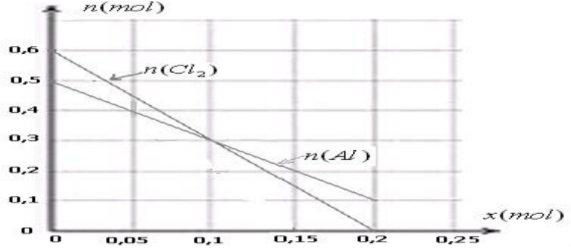
\includegraphics[width=0.5\textwidth]{./img/img01.png}\\
1) Ecrire puis équilibrer l’équation de la réaction et tracer le tableau d’avancement correspondant.\\
2) Compléter le graphe en représentant la variation de la quantité de matière du chlorure d’aluminium en fonction
de l’avancement et donner la composition finale du mélange.

\section{Détermination de la pression d’un gaz résultant d’une réaction chimique : }
\subsection{Expérience : }

On introduit une masse $m = 32,7mg$ de zinc en poudre dans un flacon à la température $\theta = 20^{circ}C$ et sous la pression atmosphérique $P_{atm} = 1013hpa$ puis on verse dans le flacon de volume 500mL un volume V=10mL d’une solution d’acide chlorhydrique de concentration c=0,5mol/L .
On donne l'équation de réaction qui se produit dans le flacon : 
$Zn_{(s)} + 2H^{+}_{(aq)} \rightarrow Zn^{2+}_{(aq)} + H_{2_{(g)}}$

\subsection{ Prévoir l’état final:  }
On peut prévoir la pression finale du gaz dihydrogène qui se produit à la fin de cette réaction par l’une des deux méthodes
suivantes : 
\\-Soit en utilisant un appareil de mesure de la pression.\\
-ou bien théoriquement en utilisant le tableau d’avancement de la réaction.


*1ère méthode : On détermine la valeur de la pression final Pf à la fin de la réaction à l’aide d’un capteur de pression,
on trouve : Pf=1038hPa

*2ème méthode : 
la quantité de matière de zinc initiale: $n_0(Zn) = \frac{m}{M} = \frac{32.7 10^{-3}}{65.4} = 0.5mmol$\\
la quantité de matière de $H^+$ initiale: $n_0(H^+) = C.V = 0.5.10.10^{-3} =  5mmol$\\

Tableau d'avancement : 

% table dont forget 
\begin{tabular}{|c|c|c|c|c|c|}
    \hline
    \multicolumn{2}{|c|}{Equation de la réaction}& \multicolumn{4}{c|}{${ Zn + 2H^+   \rightarrow Zn^{2+} + H_2}$}\\\hline
    états  & avancement& \multicolumn{4}{|c|}{quantité de Matière en mol}\\\hline
    Etat initial          &    0        &  0.5              &   5            & $ 0$       & $ 0$ \\\hline
    Etat de transformation&    $x$      & $0.5 - x$         & $ 5 - 2x$       & $x$        & $x$ \\\hline
    Etat final            &    $x_{max}$& $ 0.5 - x_{max}$  & $ 5 - 2 x_{max}$& $x_{max}$  & $ x_{max}$ \\\hline
   % \cline{2-4}\
\end{tabular}

-supposons que Zn est le réactif limitant : $0.5 - x_{max} = 0 \rightarrow x_{max} = 0.5mmol$
-supposons que $H^+$ est le réactif limitant : $5-2x_{max} = 0 \rightarrow x_{max} = 2.5mmol$
 On a  $0.5 < 2.5$

On sait que le réactif limitant est celui utilisé par défaut, donc $x_{max} = 0.5mmol$ et c’est Zn qui est limitant.

A partir du tableau d’avancement on a :$ n_{f(H_2)} =x_{max}=0,5m.mol$
En appliquant la relation des gaz parfaits au gaz dihydrogène qui occupe le volume restant du flacon :
$V_{(H_2)}=500-10=490mL$ donc $P_{(H_2)}.V_{(H_2)} = n_{(H_2)}.R.T \rightarrow P_{(H_2)} = 2485.7Pa = 25hP
$

La pression finale du dihydrogène H2 dans le flacon : $P_f = P_{(H_2)} + P_{atm}  = 25 + 1013 = 1038hPa$

\end{document}
